\begin{lemma}
    {\em Lehmann–Scheffé theorem :} If $T$ is a complete sufficient statistic for $\theta$ and 
    \begin{align}
    \label{stats/2/eqn 2.0.1}
    E(g(T)) = \tau(\theta)
    \end{align}
    then $g(T)$ is the uniformly minimum-variance unbiased estimator (UMVUE) of $\tau(\theta)$.
    
\end{lemma}




We know that 
\begin{align}
T = \sum_{i=1}^{n} X_i
\end{align}
is a complete and sufficient statistic. By the law of total expectation, 
\begin{align}
\label{stats/2/eqn 2.0.3}
E\brak{E(X_{(1)} | T )} = E(X_{(1)})
\end{align}
By Lehmann–Scheffé theorem, with
\begin{align}
\theta &= X_{(1)},\\ 
\tau(x) &= E(x),\\
g(T) &= E(X_{(1)} | T).
\end{align}
it follows from \eqref{stats/2/eqn 2.0.3} that $E(X_{(1)} | T)$ is the UMVUE of $E(X_{(1)})$.
\begin{align}
\pr{X_{(1)} > x} &= \pr{X_1 > x}\ldots \pr{X_n > x}\\
&= (1-F_{X_{1}}(x))\ldots(1-F_{X_{n}}(x))\\
&= (1-F_{X_{1}}(x))^n \\
&= \exp\brak{-\frac{nx}{\theta}}\\
F_{X_{(1)}}(x) &= 1 - \exp\brak{-\frac{nx}{\theta}}\\
f_{X_{(1)}}(x) &= \frac{n}{\theta} \exp\brak{-\frac{nx}{\theta}}
\end{align}
Therefore, $X_{(1)}$ follows an exponential distribution with mean $\dfrac{\theta}{n}$.
\begin{align}
E(X_{(1)}) = \frac{\theta}{n}
\end{align}
Note that,
\begin{align}
E\brak{\frac{T}{n^2}} &= E\brak{\frac{\sum_{i=1}^n X_i}{n^2}}\\
&= \frac{E(\sum_{i=1}^n X_i)}{n^2}\\
&= \sum_{i=1}^n \frac{E(X_i)}{n^2}\\
&= \sum_{i=1}^n \frac{\theta}{n^2}\\
&= \frac{\theta}{n}\\
&= E(X_{(1)})
\end{align}
Therefore, by Lehmann–Scheffé theorem, with
\begin{align}
\theta &= X_{(1)},\\
\tau(x) &= E(x),\\
g(T) &= \frac{T}{n^2},
\end{align}
it follows that $\dfrac{T}{n^2}$ is UMVUE of $E(X_{(1)})$.\\

Since there exists a unique UMVUE for $E(X_{(1)})$, it follows that 
\begin{align}
E(X_{(1)} | T) = \frac{T}{n^2}
\end{align}
Hence, option A is correct.
\begin{figure}[!hbt]
    \centering
	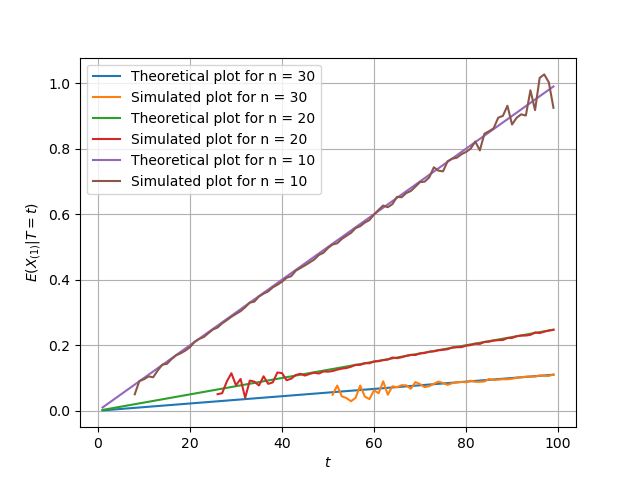
\includegraphics[width=\columnwidth]{stats/solutions/2/Figures/Figure_1.png}
    \caption{Theory vs Simulated plot of $E(X_{(1)} |T)$}
    \label{stats/2/CDF_Y}
\end{figure}
